\documentclass[a4paper,11pt]{article}
\usepackage{graphicx}
\usepackage[hidelinks]{hyperref}
\setcounter{tocdepth}{1}
\begin{document}
\begin{center}

\Huge\textbf{Functional Requirements\\}
																											
\vspace{2 cm}

\LARGE\textbf{Group Name:} Group 6\_b\newline
 
\vspace{0.5 cm}
\begin{tabular}{lr}
Jessica (JI) Lessev&13049136\\
Thabang (TM) Letageng&13057937\\
Michelle Swanepoel&13066294\\
Prenolan Govender&13102380\\
Fako (FJA) Peleha&12230830\\
Lutfiyya Razak&10198408\\
Ephiphania Munava&10624610\\
Maria Qumalo&29461775\\
\end{tabular}

\vspace{1cm}
\textbf{Git repository link:\\}
\url{https://github.com/u12230830/COS301\_6b}

\vspace{1cm}
\textbf{Date:} 27 February 2015
\end{center}


\newpage

\tableofcontents
\newpage
\setlength{\voffset}{-3cm}
\hspace{-1cm}The following modules will be discussed, each with their own set of use cases:
\begin{itemize}
	\item BuzzSpace Handling
	\item Thread Handling
	\item Posts Handling
	\item Filtering 
	\item Authorisation
	\item Reporting
	\item Profile Handling
\end{itemize}
\newpage
\setlength{\voffset}{-3cm}

\begin{center}
\section*\textbf\huge{BuzzSpace Handling}
\addcontentsline{toc}{section}{BuzzSpace Handling}
\\
\Large{Use Cases}
\end{center}

%-------------------------------------------------------START EDITING HERE FOR BUZZSPACE HANDLING------------------------------------------------------------
%MICHELLE
\section{Create BuzzSpace}
\subsection*{Description:}
\subsection{Prioritization:}
\subsection{Conditions and Data Structures:}
\subsubsection*{Pre-Conditions:}
\subsubsection*{Post-Conditions:}
\subsubsection*{Requests and Results Data Structures:}
\subsection{Required Functionality:} 
\subsection{Process Specifications:} 

%MICHELLE
\section{Read BuzzSpace}
\subsection*{Description:}
\subsection{Prioritization:} 
\subsection{Conditions and Data Structures:}
\subsubsection*{Pre-Conditions:}
\subsubsection*{Post-Conditions:}
\subsubsection*{Requests and Results Data Structures:}
\subsection{Required Functionality:} 
\subsection{Process Specifications:} 

%MICHELLE
\section{Update BuzzSpace}
\subsection*{Description:}
\subsection{Prioritization:} 
\subsection{Conditions and Data Structures:}
\subsubsection*{Pre-Conditions:}
\subsubsection*{Post-Conditions:}
\subsubsection*{Requests and Results Data Structures:}
\subsection{Required Functionality:} 
\subsection{Process Specifications:} 

%MICHELLE
\section{Delete BuzzSpace}
\subsection*{Description:}
\subsection{Prioritization:} 
\subsection{Conditions and Data Structures:}
\subsubsection*{Pre-Conditions:}
\subsubsection*{Post-Conditions:}
\subsubsection*{Requests and Results Data Structures:}
\subsection{Required Functionality:} 
\subsection{Process Specifications:} 

%LEAVE
\newpage
\begin{center}
\section*\textbf\huge{Thread Handling}
\addcontentsline{toc}{section}{Thread Handling}
\\
\Large{Use Cases}
\end{center}
\setcounter{section}{0}

%-------------------------------------------------------START EDITING HERE FOR THREAD HANDLING------------------------------------------------------------
%JESSICA
\section{Create Thread}
\subsection*{Description:}
1.	User activates “Create Thread” function by selecting the “Create Thread” option.\\
2.	System responds by presenting user with a form to create thread topic etc\\
3.	User fills in form  topic of thread, tags, etc and submits the form\\
4.	System reviews the submitted information and  verifies users status and privileges, decorates the thread as needed and checks that all requirements (rules) are followed by the user based on his/her status\\
5.	 System displays either an acknowledgement or error message based on the pervious checkpoint.
\subsection{Prioritization:} 
This Use case is considered Important
\subsection{Conditions and Data Structures:}
Participants:
Initiated by User and communicates with system
\subsubsection*{Pre-Conditions:}
1.	The User is logged in \\
a.	The user has a specific status
\subsubsection*{Post-Conditions:}
1.	The user fills in the form to create a new thread\\
a.	User must have a specific status in order to perform certain functions when creating a thread
\subsubsection*{Requests and Results Data Structures:}
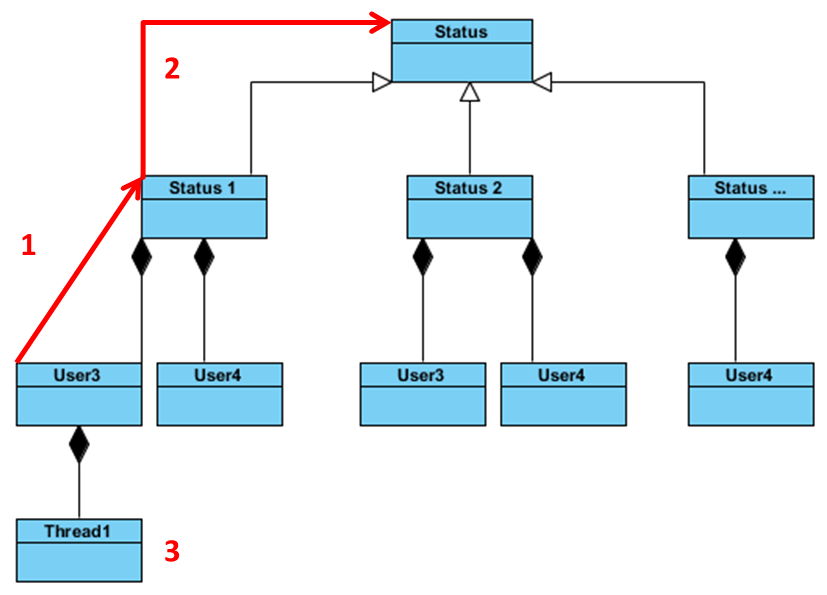
\includegraphics{./Images/CRUDThread/Diagrams/1.png}
Status can be an abstract class and each sub-class will be a generalization of this class as each new status “IS-A” status.
Each user “HAS-A” status and thus each new user will be a composition of each specific status class.
Each thread “HAS-A” user that started it and thus each new thread will be a composition of each user.\\\\
Steps:\\\\
1.	If the user attempts to create a thread, the system will first check if the user is logged in.\\
1.1.	If so, it will go to number 1 above and check the users status\\
1.1.1.	The system verifies the status and at number 2 checks that the user has the privileges to create threads of the appropriate size, contents etc.\\
1.1.1.1	If the user has the necessary privileges then the thread is created at 3\\
1.1.1.2	Otherwise an error message is displayed telling the user that he/she does not have the necessary privileges \\
2.	If the user is not logged in, an error message is displayed telling the user that he/she is not logged in and it will redirect to the logging page.\\
\subsection{Required Functionality:} 
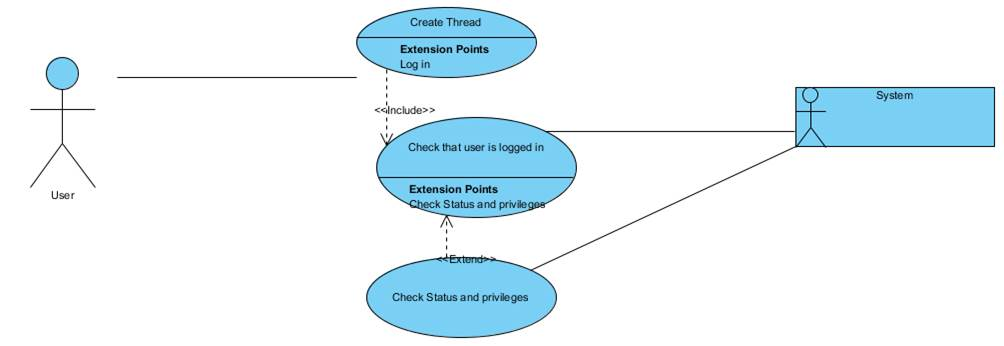
\includegraphics[width=1\linewidth]{./Images/CRUDThread/Diagrams/2.jpg}\\
\subsection{Process Specifications:} 
Activity Diagram\\
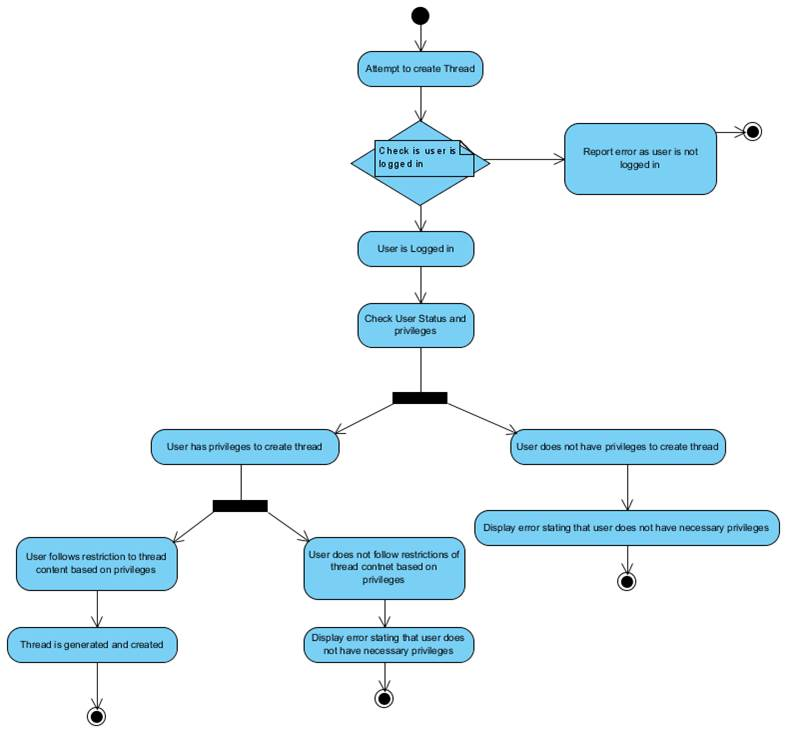
\includegraphics[width=1\linewidth]{./Images/CRUDThread/Diagrams/3.jpg}\\
\newpage
Sequence Diagram\\
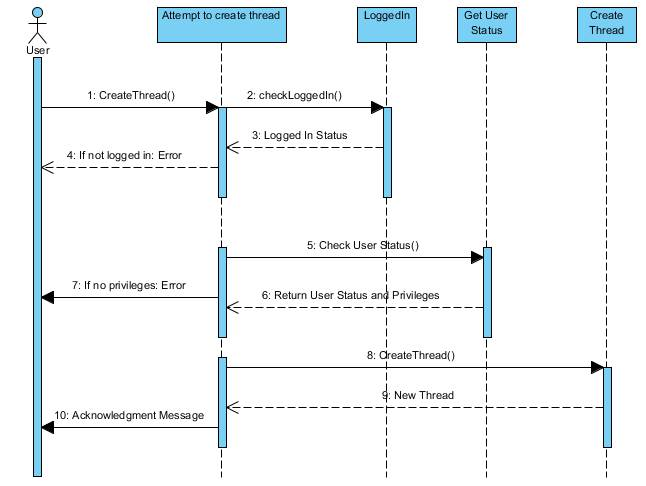
\includegraphics[width=1\linewidth]{./Images/CRUDThread/Diagrams/4.jpg}\\

%JESSICA
\section{Read Thread}
\subsection*{Description:}
1.	User activates “Read Thread” function by selecting the “A Thread” they wish to read.\\
2.	System responds by presenting user with the selected thread of posts\\
3.	User reads the posts and based on privileges can make changes such as update, delete, reply, tag, rate etc\\

\subsection{Prioritization:}
This Use case is considered Important\\ 
\subsection{Conditions and Data Structures:}
Participants:\\
Initiated by User and communicates with system\\
\subsubsection*{Pre-Conditions:}
1.	The user must click on a thread they wish to read\\
1.1.	If User is logged in and\\
1.1.1.	User has status with high privileges then the user has options to change thread\\
1.1.1.1.	Calls other use cases\\
1.1.2.	Otherwise user is automatically logged in as “Guest” and can only view posts
\subsubsection*{Post-Conditions:}
1.	System displays selected thread with posts\\
2.	If user is logged on and has privileges then an attempt to make changes such as update, delete, reply, tag, rate etc will be acknowledged. 

\subsubsection*{Requests and Results Data Structures:}
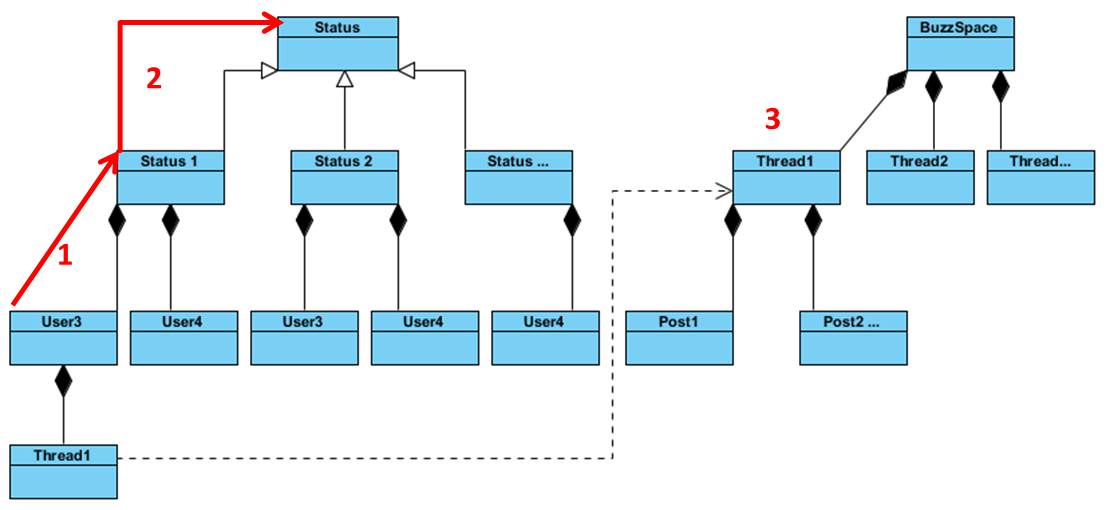
\includegraphics[width=1\linewidth]{./Images/CRUDThread/Diagrams/5.jpg}\\
Status can be an abstract class and each sub-class will be a generalization of this class as each new status “IS-A” status.\\
Each user “HAS-A” status and thus each new user will be a composition of each specific status class.\\
Each thread “HAS-A” user that started it and thus each new thread will be a composition of each user.\\
Each thread “HAS-A” BuzzSpace and thus each new thread will be a composition of each BuzzSpace.\\
Each Post “HAS-A” Thread and thus each new post will be a composition of each Thread\\\\

Steps:\\
1.	If the user attempts to enter a thread to read then the system will first check if the user is logged in.\\
1.1.	If so it will go to number 3 and open the selected thread to read.\\
1.1.1.	If user attempts to alter a post it will go to number 1 above and check the users status\\
1.1.1.1.	The system verifies the status and at number 2 checks that the user has the privileges to create threads of the appropriate size, contents etc.\\
1.1.1.2.	If the user has the necessary privileges then the post is altered at 3\\
1.1.1.3.	Otherwise an error message is displayed telling the user that he/she does not have the necessary privileges \\
1.2.	If not the user will be automatically logged on as “Guest”


\subsection{Required Functionality:} 
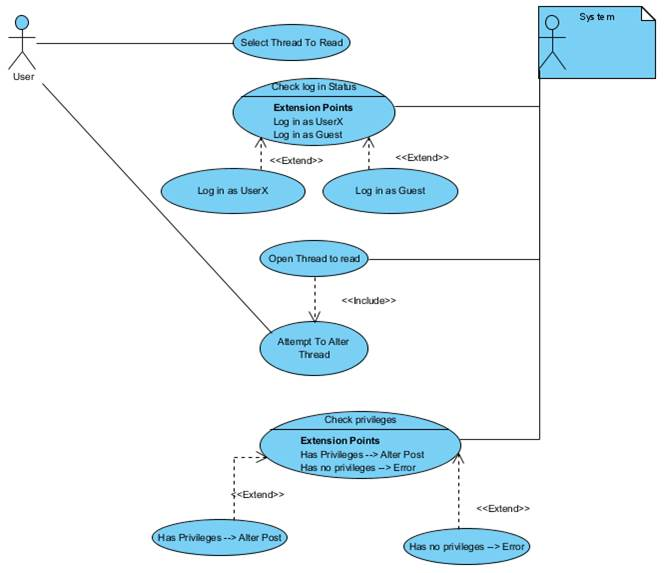
\includegraphics[width=1\linewidth]{./Images/CRUDThread/Diagrams/6.jpg}\\
\subsection{Process Specifications:} 
Activity Diagram\\
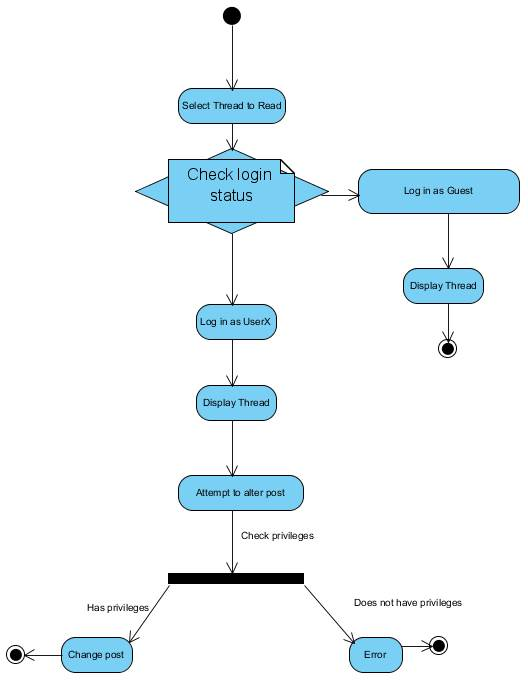
\includegraphics[width=1\linewidth]{./Images/CRUDThread/Diagrams/7.jpg}\\
\newpage
Sequence Diagram\\
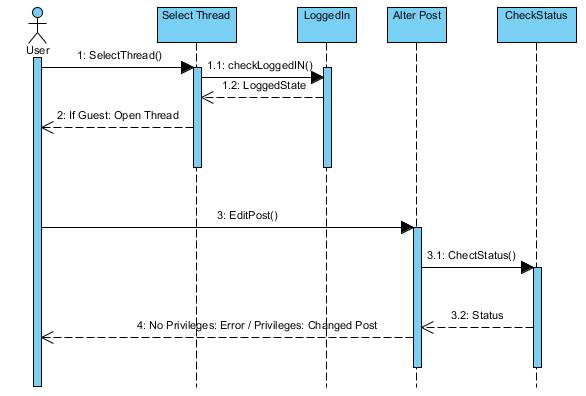
\includegraphics[width=1\linewidth]{./Images/CRUDThread/Diagrams/8.jpg}\\

%JESSICA
\section{Update Thread}
\subsection*{Description:}
1.	User activates “Update Thread” function by selecting the “Update Thread” option by choosing how they wish to update the thread.\\
2.	System checks to see whether user is logged in\\
3.	System reviews the submitted information and  verifies users status and privileges, decorates the thread as needed and checks that all requirements (rules) are followed by the user based on his/her status\\
4.	 System displays either an acknowledgement or error message based on the pervious checkpoint.\\

\subsection{Prioritization:} 
This Use case is considered Important\\
\subsection{Conditions and Data Structures:}
Participants:\\
Initiated by User and communicates with system\\
\subsubsection*{Pre-Conditions:}
1.	User chooses the way in which to update a thread\\
2.	The User is logged in \\
2.1.	The user has a specific status\\
2.2.	User must have a specific status in order to perform certain functions when updating a thread\\
\subsubsection*{Post-Conditions:}
1.	System displays an acknowledgement message and updates  the new thread  if user follows “status based rules”\\
2.	Systems display an error message and requests user to restart if user attempts to perform a function that is not within the scope of their status privileges.\\
\subsubsection*{Requests and Results Data Structures:}
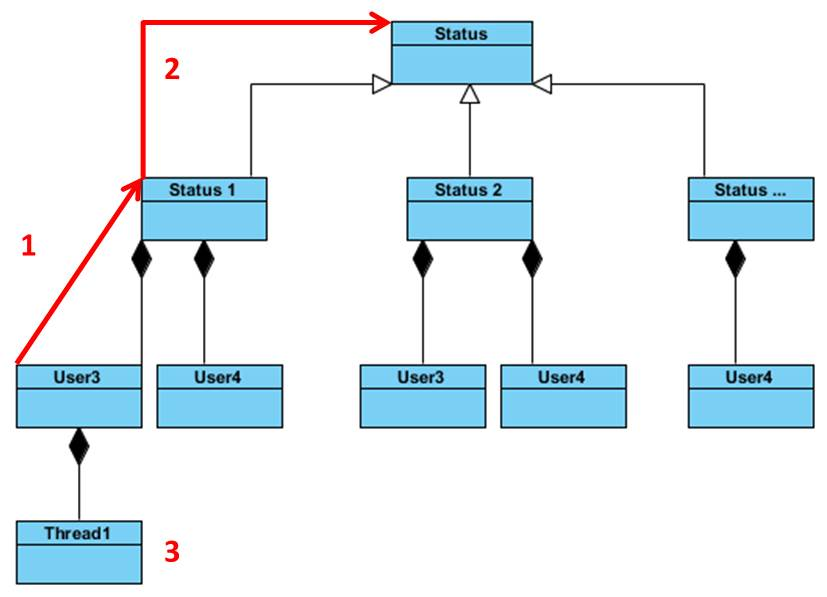
\includegraphics[width=1\linewidth]{./Images/CRUDThread/Diagrams/9.jpg}\\
Status can be an abstract class and each sub-class will be a generalization of this class as each new status “IS-A” status.\\
Each user “HAS-A” status and thus each new user will be a composition of each specific status class.\\
Each thread “HAS-A” user that started it and thus each new thread will be a composition of each user.\\
Steps:\\
1.	If the user attempts to update a thread, the system will first check if the user is logged in.\\
1.1.	If so, it will go to number 1 above and check the users status\\
1.1.1.	The system verifies the status and at number 2 checks that the user has the privileges to update threads in the specific way chosen.\\
1.1.1.1.	If the user has the necessary privileges then the thread is updated at 3\\
1.1.1.2.	Otherwise an error message is displayed telling the user that he/she does not have the necessary privileges \\
1.2.	If the user is not logged in, an error message is displayed telling the user that he/she is not logged in and it will redirect to the logging page.\\
\subsection{Required Functionality:}
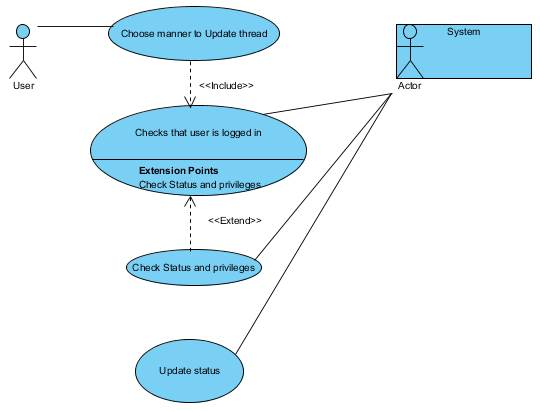
\includegraphics[width=1\linewidth]{./Images/CRUDThread/Diagrams/10.jpg}\\
\subsection{Process Specifications:} 
Activity Diagram\\
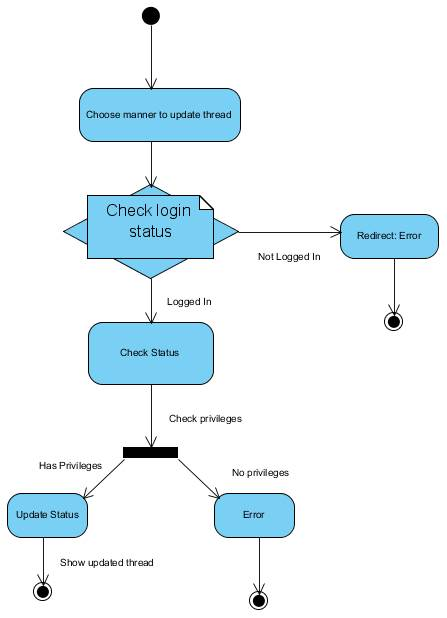
\includegraphics[width=1\linewidth]{./Images/CRUDThread/Diagrams/11.jpg}\\
\newpage
Sequence Diagram\\
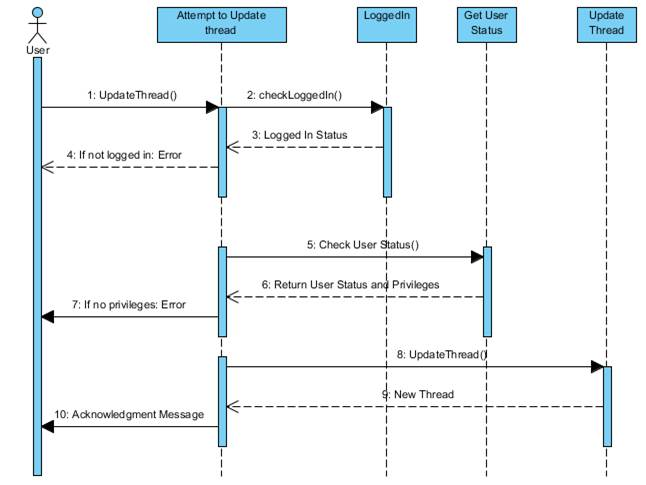
\includegraphics[width=1\linewidth]{./Images/CRUDThread/Diagrams/12.jpg}\\

%JESSICA
\section{Delete Thread}
\subsection*{Description:}
1	User activates “Delete Thread” function by selecting the “Delete Thread” option.\\
2	System checks to see whether user is logged in\\
3	System reviews the submitted information and  verifies users status and privileges\\
4	System displays either an acknowledgement and removes the thread or displays an error message based on the pervious checkpoint.\\
\subsection{Prioritization:} 
This Use case is considered Important\\
\subsection{Conditions and Data Structures:}
Participants:\\
Initiated by User and communicates with system\\
\subsubsection*{Pre-Conditions:}
1.	User selects “Delete Thread” \\
2.	The User is logged in \\
2.1.	The user has a specific status\\
2.2.	User must have a specific status in order to delete a thread\\
\subsubsection*{Post-Conditions:}
1.	System displays an acknowledgement message and removes  the thread  if user follows “status based rules”\\
2.	Systems display an error message and requests user to restart if user attempts to perform a function that is not within the scope of their status privileges.\\
\subsubsection*{Requests and Results Data Structures:}
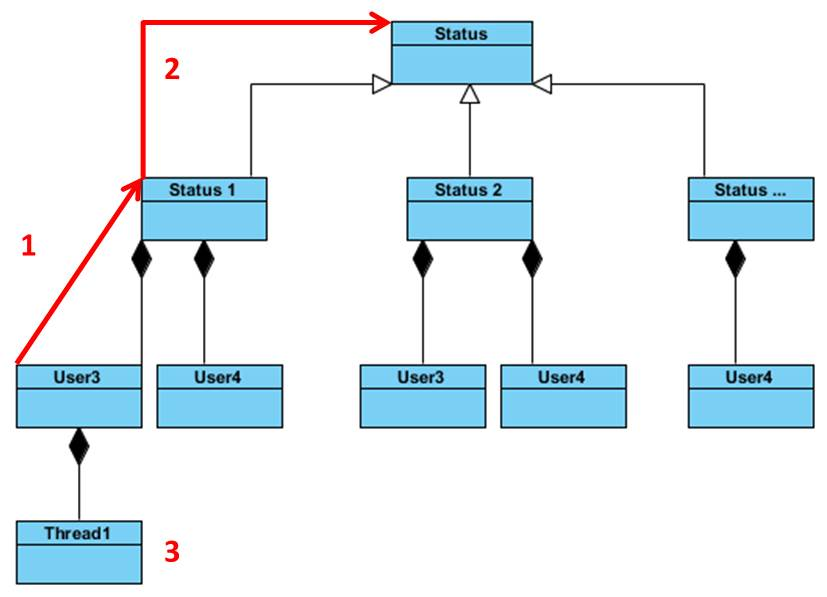
\includegraphics[width=1\linewidth]{./Images/CRUDThread/Diagrams/13.jpg}\\
Status can be an abstract class and each sub-class will be a generalization of this class as each new status “IS-A” status.\\
Each user “HAS-A” status and thus each new user will be a composition of each specific status class.\\
Each thread “HAS-A” user that started it and thus each new thread will be a composition of each user.\\
Steps:\\
1.	If the user attempts to delete a thread, the system will first check if the user is logged in.\\
1.1.	If so, it will go to number 1 above and check the users status\\
1.1.1.	The system verifies the status and at number 2 checks that the user has the privileges to delete thread.\\
1.1.1.1.	If the user has the necessary privileges then the thread at 3 is removed from the tree\\
1.1.1.2.	Otherwise an error message is displayed telling the user that he/she does not have the necessary privileges \\
1.2.	If the user is not logged in, an error message is displayed telling the user that he/she is not logged in and it will redirect to the logging page.\\
\subsection{Required Functionality:} 
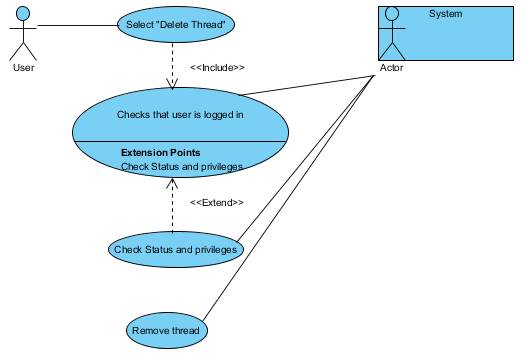
\includegraphics[width=1\linewidth]{./Images/CRUDThread/Diagrams/14.jpg}\\
\subsection{Process Specifications:} 
Activity Diagram\\
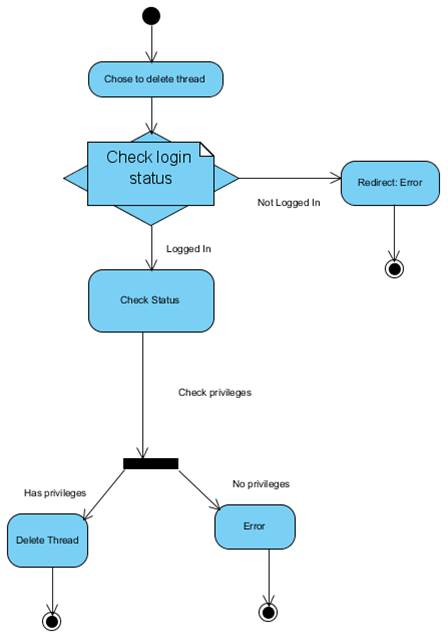
\includegraphics[width=1\linewidth]{./Images/CRUDThread/Diagrams/15.jpg}\\
\newpage
Sequence Diagram\\
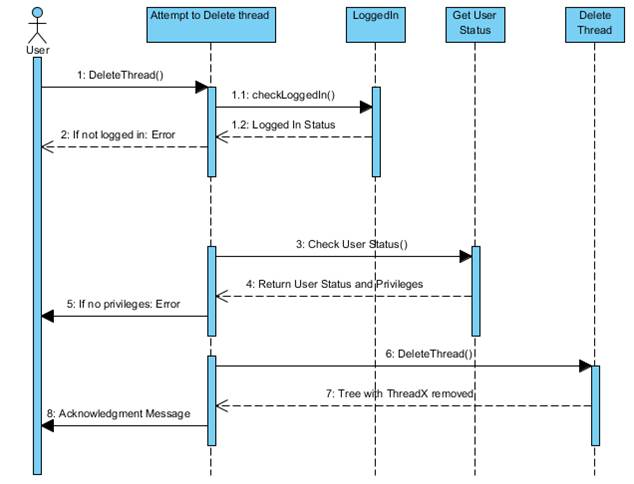
\includegraphics[width=1\linewidth]{./Images/CRUDThread/Diagrams/16.jpg}\\

%JIMMY
\section{Summarise Thread}
\subsection*{Description:}
\subsection{Prioritization:} 
\subsection{Conditions and Data Structures:}
\subsubsection*{Pre-Conditions:}
\subsubsection*{Post-Conditions:}
\subsubsection*{Requests and Results Data Structures:}
\subsection{Required Functionality:} 
\subsection{Process Specifications:} 

%JIMMY
\section{Hide Thread}
\subsection*{Description:}
\subsection{Prioritization:} 
\subsection{Conditions and Data Structures:}
\subsubsection*{Pre-Conditions:}
\subsubsection*{Post-Conditions:}
\subsubsection*{Requests and Results Data Structures:}
\subsection{Required Functionality:} 
\subsection{Process Specifications:} 

%JIMMY
\section{Close Thread}
\subsection*{Description:}
\subsection{Prioritization:} 
\subsection{Conditions and Data Structures:}
\subsubsection*{Pre-Conditions:}
\subsubsection*{Post-Conditions:}
\subsubsection*{Requests and Results Data Structures:}
\subsection{Required Functionality:} 
\subsection{Process Specifications:} 

%JIMMY
\section{Move Thread}
\subsection*{Description:}
\subsection{Prioritization:} 
\subsection{Conditions and Data Structures:}
\subsubsection*{Pre-Conditions:}
\subsubsection*{Post-Conditions:}
\subsubsection*{Requests and Results Data Structures:}
\subsection{Required Functionality:} 
\subsection{Process Specifications:} 

%LEAVE
\newpage
\begin{center}
\section*\textbf\huge{Post Handling}
\addcontentsline{toc}{section}{Post Handling}
\\
\Large{Use Cases}
\end{center}
\setcounter{section}{0}
%---------------------------------------------------------------START EDITING HERE FOR POST HANDLING----------------------------------------------------------------------
%MICHELLE
\section{Create Post}
\subsection*{Description:}
\subsection{Prioritization:} 
\subsection{Conditions and Data Structures:}
\subsubsection*{Pre-Conditions:}
\subsubsection*{Post-Conditions:}
\subsubsection*{Requests and Results Data Structures:}
\subsection{Required Functionality:} 
\subsection{Process Specifications:} 

%MICHELLE
\section{Read Post}
\subsection*{Description:}
\subsection{Prioritization:} 
\subsection{Conditions and Data Structures:}
\subsubsection*{Pre-Conditions:}
\subsubsection*{Post-Conditions:}
\subsubsection*{Requests and Results Data Structures:}
\subsection{Required Functionality:} 
\subsection{Process Specifications:} 

%MICHELLE
\section{Update Post}
\subsection*{Description:}
\subsection{Prioritization:} 
\subsection{Conditions and Data Structures:}
\subsubsection*{Pre-Conditions:}
\subsubsection*{Post-Conditions:}
\subsubsection*{Requests and Results Data Structures:}
\subsection{Required Functionality:} 
\subsection{Process Specifications:} 

%MICHELLE
\section{Delete Post}
\subsection*{Description:}
\subsection{Prioritization:} 
\subsection{Conditions and Data Structures:}
\subsubsection*{Pre-Conditions:}
\subsubsection*{Post-Conditions:}
\subsubsection*{Requests and Results Data Structures:}
\subsection{Required Functionality:} 
\subsection{Process Specifications:} 

%PRENOLAN
\section{Mark solution post}
\subsection*{Description:}
\subsection{Prioritization:} 
\subsection{Conditions and Data Structures:}
\subsubsection*{Pre-Conditions:}
\subsubsection*{Post-Conditions:}
\subsubsection*{Requests and Results Data Structures:}
\subsection{Required Functionality:} 
\subsection{Process Specifications:} 

%PRENOLAN
\section{Evaluate Posts}
\subsection*{Description:}
\subsection{Prioritization:} 
\subsection{Conditions and Data Structures:}
\subsubsection*{Pre-Conditions:}
\subsubsection*{Post-Conditions:}
\subsubsection*{Requests and Results Data Structures:}
\subsection{Required Functionality:} 
\subsection{Process Specifications:} 

%PRENOLAN
\section{Post Voting}
\subsection*{Description:}
\subsection{Prioritization:} 
\subsection{Conditions and Data Structures:}
\subsubsection*{Pre-Conditions:}
\subsubsection*{Post-Conditions:}
\subsubsection*{Requests and Results Data Structures:}
\subsection{Required Functionality:} 
\subsection{Process Specifications:} 

%MARIA
\section{Post Tagging}
\subsection*{Description:}
One very important functional requierment is the ability for the user to structure the information and content comming in according to his own preferance and needs. Socilal tagging will enable him to do so.
\subsection{Prioritization:} 
\subsection{Conditions and Data Structures:}
\subsubsection*{Pre-Conditions:}
\subsubsection*{Post-Conditions:}
\subsubsection*{Requests and Results Data Structures:}
\subsection{Required Functionality:} 
\subsection{Process Specifications:} 

%LEAVE
\newpage
\begin{center}
\section*\textbf\huge{Filtering}
\addcontentsline{toc}{section}{Filtering}
\\
\Large{Use Cases}
\end{center}
\setcounter{section}{0}
%---------------------------------------------------------------START EDITING HERE FOR FILTERING----------------------------------------------------------------------
%THABANG
\section{Filter threads and buzzspaces}
\subsection*{Description:}
\subsection{Prioritization:} 
\subsection{Conditions and Data Structures:}
\subsubsection*{Pre-Conditions:}
\subsubsection*{Post-Conditions:}
\subsubsection*{Requests and Results Data Structures:}
\subsection{Required Functionality:} 
\subsection{Process Specifications:} 

%THABANG
\section{Filter threads and buzzspaces}
\subsection*{Description:}
\subsection{Prioritization:} 
\subsection{Conditions and Data Structures:}
\subsubsection*{Pre-Conditions:}
\subsubsection*{Post-Conditions:}
\subsubsection*{Requests and Results Data Structures:}
\subsection{Required Functionality:} 
\subsection{Process Specifications:} 

%LEAVE
\newpage
\begin{center}
\section*\textbf\huge{Authorisation}
\addcontentsline{toc}{section}{Authorisation}
\\
\Large{Use Cases}
\end{center}
\setcounter{section}{0}
%---------------------------------------------------------------START EDITING HERE FOR AUTHORISATION----------------------------------------------------------------------
%MICHELLE
\section{Login}
\subsection*{Description:}
\subsection{Prioritization:} 
\subsection{Conditions and Data Structures:}
\subsubsection*{Pre-Conditions:}
\subsubsection*{Post-Conditions:}
\subsubsection*{Requests and Results Data Structures:}
\subsection{Required Functionality:} 
\subsection{Process Specifications:} 

%JESSICA
\section{Logout}
\subsection*{Description:}
1.	User activates “Logout” function by selecting the “Logout” option.\\
2.	System responds by presenting user with standard Guest interface with no profile or privileges\\
\subsection{Prioritization:}
This Use case is considered Important\\ 
\subsection{Conditions and Data Structures:}
Participants:\\
Initiated by User and communicates with system\\
\subsubsection*{Pre-Conditions:}
1.	The user must click on “Logout” function\\
\subsubsection*{Post-Conditions:}
1.	System displays user with standard guest interface\\
2.	User has no privileges and status and cannot perform any function that a logged in user can\\
\subsubsection*{Requests and Results Data Structures:}
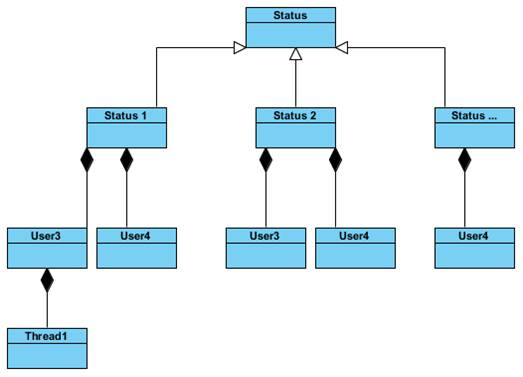
\includegraphics[width=1\linewidth]{./Images/CRUDThread/Diagrams/17.jpg}\\
Steps:\\
1.	User selects the logout option\\
1.1.	Boolean field in the specific user class – e.g User3 will be switched to false\\
2.	User will be presented with Guest interface\\
\subsection{Required Functionality:} 
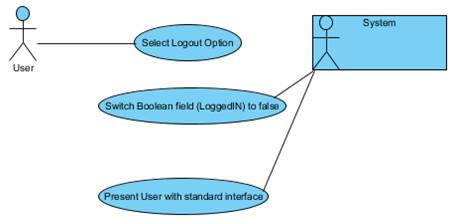
\includegraphics[width=1\linewidth]{./Images/CRUDThread/Diagrams/18.jpg}\\
\subsection{Process Specifications:} 
Activity Diagram\\
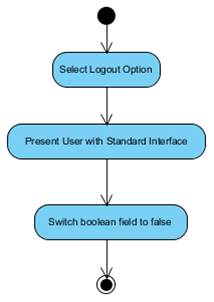
\includegraphics[width=1\linewidth]{./Images/CRUDThread/Diagrams/19.jpg}\\
Sequence Diagram\\
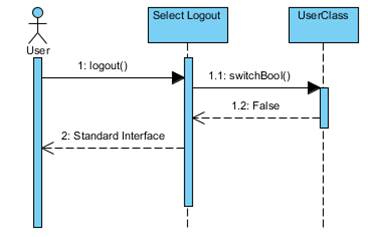
\includegraphics[width=1\linewidth]{./Images/CRUDThread/Diagrams/20.jpg}\\

%MICHELLE
\section{Registration}
\subsection*{Description:}
\subsection{Prioritization:} 
\subsection{Conditions and Data Structures:}
\subsubsection*{Pre-Conditions:}
\subsubsection*{Post-Conditions:}
\subsubsection*{Requests and Results Data Structures:}
\subsection{Required Functionality:} 
\subsection{Process Specifications:} 

%LEAVE
\newpage
\begin{center}
\section*\textbf\huge{Reporting}
\addcontentsline{toc}{section}{Reporting}
\\
\Large{Use Cases}
\end{center}
\setcounter{section}{0}
%---------------------------------------------------------------START EDITING HERE FOR REPORTING----------------------------------------------------------------------
%LUTFIYYA
\section{Statistical Reporting}
\subsection*{Description:}
\subsection{Prioritization:} 
\subsection{Conditions and Data Structures:}
\subsubsection*{Pre-Conditions:}
\subsubsection*{Post-Conditions:}
\subsubsection*{Requests and Results Data Structures:}
\subsection{Required Functionality:} 
\subsection{Process Specifications:} 

%LEAVE
\newpage
\begin{center}
\section*\textbf\huge{Profile Handling}
\addcontentsline{toc}{section}{Proflie Handling}
\\
\Large{Use Cases}
\end{center}
\setcounter{section}{0}
%---------------------------------------------------------------START EDITING HERE FOR PROFILE HANDLING----------------------------------------------------------------------
%EPHI
\section{Modify Profile}
\subsection*{Description:}
\textbf{Description:}Profile modification allows the user logged into the system to modify the user profile that was previously created.
\subsection{Prioritization:}
\textbf{}Important
\subsection{Conditions and Data Structures:}
\subsubsection*{Pre-Conditions:}
\textbf{}User logged into the system. 
\textbf{}User has an already existing profile. 
\subsubsection*{Post-Conditions:}
\textbf{}User modifies existing profile: User is logged in and user profile has been modified. 
\textbf{}User keeps already existing profile: User had logged into the system and the profile had not been modified. 
\subsubsection*{Requests and Results Data Structures:}
\subsection{Required Functionality:}
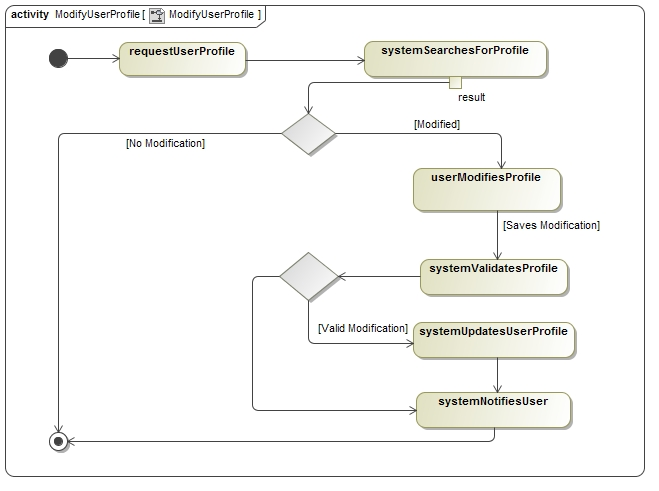
\includegraphics{Images/UserProfile/ModifyUserProfile}
\subsection{Process Specifications:} 
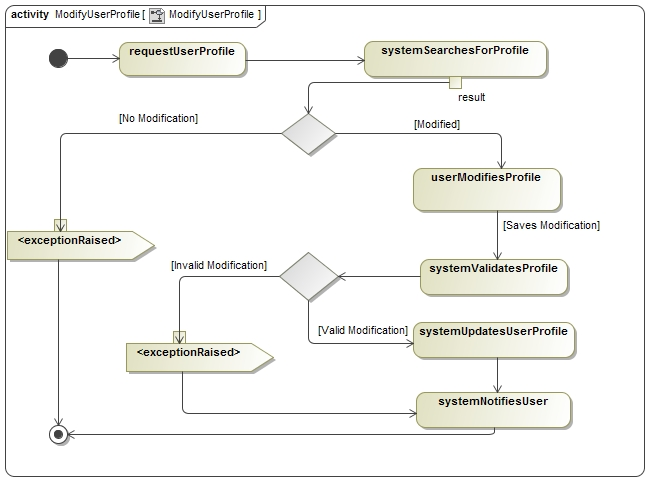
\includegraphics{Images/UserProfile/ModifyUserProfileActivity}

%EPHI
\section{Create Profile}
\subsection*{Description:}
\subsection{Prioritization:} 
\subsection{Conditions and Data Structures:}
\subsubsection*{Pre-Conditions:}
\subsubsection*{Post-Conditions:}
\subsubsection*{Requests and Results Data Structures:}
\subsection{Required Functionality:} 
\subsection{Process Specifications:} 

%.........
\section{Create Private Message}
\subsection*{Description:}
\subsection{Prioritization:} 
\subsection{Conditions and Data Structures:}
\subsubsection*{Pre-Conditions:}
\subsubsection*{Post-Conditions:}
\subsubsection*{Requests and Results Data Structures:}
\subsection{Required Functionality:} 
\subsection{Process Specifications:} 

%.........
\section{Read Private Message}
\subsection*{Description:}
\subsection{Prioritization:} 
\subsection{Conditions and Data Structures:}
\subsubsection*{Pre-Conditions:}
\subsubsection*{Post-Conditions:}
\subsubsection*{Requests and Results Data Structures:}
\subsection{Required Functionality:} 
\subsection{Process Specifications:} 

%.........
\section{Update Private Message}
\subsection*{Description:}
\subsection{Prioritization:} 
\subsection{Conditions and Data Structures:}
\subsubsection*{Pre-Conditions:}
\subsubsection*{Post-Conditions:}
\subsubsection*{Requests and Results Data Structures:}
\subsection{Required Functionality:} 
\subsection{Process Specifications:} 

%.........
\section{Delete Private Message}
\subsection*{Description:}
\subsection{Prioritization:} 
\subsection{Conditions and Data Structures:}
\subsubsection*{Pre-Conditions:}
\subsubsection*{Post-Conditions:}
\subsubsection*{Requests and Results Data Structures:}
\subsection{Required Functionality:} 
\subsection{Process Specifications:} 

%LEAVE
\newpage
\begin{center}
\section*\textbf\huge{Domain Model}
\addcontentsline{toc}{section}{Domain Model}

\end{center}
\setcounter{section}{0}
%---------------------------------------------------------------START EDITING HERE FOR DOMAIN MODEL----------------------------------------------------------------------

\end{document}

